\subsection{\label{subsec:FZV7}Auflösungsvermögen}
\textbf{\textit{Was bestimmt das Auflösungsvermögen eines Mikroskops?}} \\
$\rightarrow$
Es gibt verschiedene Ansätze, um das Auflösungsvermögen eines Mikroskops zu beschreiben,
wobei in der Fluoreszenzmikroskopie oft das Rayleigh-Kriterium verwendet wird.
Dieses Kriterium legt fest, wann zwei fluoreszierende oder leuchtende Punkte voneinander
getrennt beobachtbar sind. Da durch die Abbildung durch eine kreisförmige (Linsen-)Blende
Beugungsscheibchen (Airy-Scheibchen) statt punktförmiger Intensitäten beobachtet werden (siehe Abb.~\ref{fig:airy}),
definiert das Rayleigh-Kriterium zwei leuchtende Punkte als getrennt beobachtbar,
wenn das Intensitätsmaximum des einen Signals in das erste Minimum des anderen fällt.
Die schwächste Intensität zwischen den Punkten beträgt dann $73,5\%$ der Maximalintensität,
was auch als verallgemeinertes Rayleigh-Kriterium bekannt ist. \\
Für die klassische Fluoreszenzmikroskopie lässt sich der minimale Abstand $d$ zwischen zwei Punkten,
die das Rayleigh-Kriterium erfüllen, wie folgt quantifizieren
\begin{equation}\label{eq:aufl}
  d = \frac{0,61\,\lambda}{\text{NA}},
\end{equation}
wobei $\lambda$ die Wellenlänge der Fluoreszenz beschreibt.
Im theoretischen Idealfall ergibt sich für den konfokalen Aufbau eine weitere
Verbesserung aufgrund der Lochblende, was jedoch nur einer Verringerung des Vorfaktors entspricht. \\
Insgesamt zeigt sich, dass das Auflösungsvermögen eines Mikroskops proportional zur untersuchten
Wellenlänge und invers proportional zur numerischen Apertur des Detektionsobjektivs ist \cite{Auf1, Auf2, Auf3}.
\begin{figure}[h!]
  \centering
  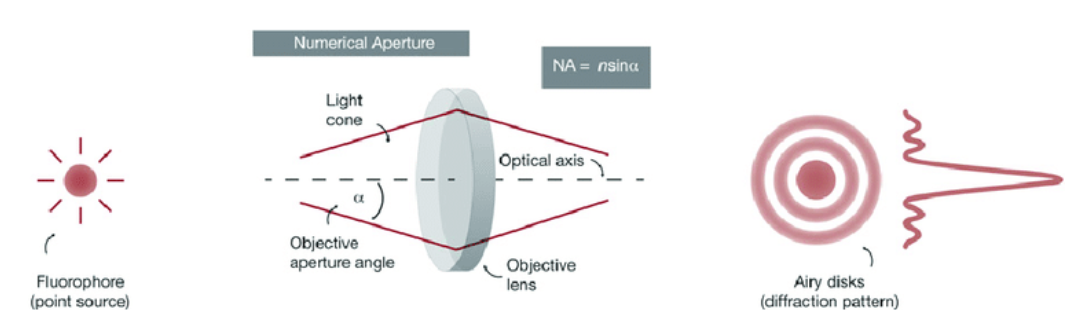
\includegraphics[width=0.6\textwidth]{psf.png}
  \caption{\label{fig:airy}Schematische Darstellung der Airy-Scheibchen, die durch
    Beugung an einer kreisförmigen Blende entstehen. Die Intensität (rechts) zeigt die
    Point-spread-function des abbildenden Systems. Die Grafik wurde Ref.~\cite{psf} entnommen.}
\end{figure} \FloatBarrier